% -*- mode: noweb; noweb-default-code-mode: R-mode; -*-

\documentclass[article]{jss}
\usepackage{amsmath}

%\usepackage[]{amsmath, amsfonts, amstext, amsthm} 
%\usepackage{amssymb}
%\usepackage[]{graphics} 
%\usepackage{epsfig}
%\usepackage{epstopdf}

%%%%%%%%%%%%%%%%%%%%%%%%%%%%%%
%% declarations for jss.cls %%%%%%%%%%%%%%%%%%%%%%%%%%%%%%%%%%%%%%%%%%
%%%%%%%%%%%%%%%%%%%%%%%%%%%%%%

%% almost as usual
\author{Ingmar Visser\\University of Amsterdam \And 
        Maarten Speekenbrink\\University College London}
        
\title{\pkg{depmixS4} : An \proglang{R}-package for hidden Markov models}


%% for pretty printing and a nice hypersummary also set:
\Plainauthor{Ingmar Visser, Maarten Speekenbrink} %% comma-separated
\Plaintitle{depmixS4: An R-package for hidden Markov models} %% without formatting

\Shorttitle{depmixS4: Hidden Markov Models} %% a short title (if necessary)

%% an abstract and keywords
\Abstract{
	
	\pkg{depmixS4} implements a general framework for defining and
	estimating dependent mixture models in the \proglang{R}
	programming language \citep{R2009}.  This includes standard Markov
	models, latent/hidden Markov models, and latent class and finite
	mixture distribution models.  The models can be fitted on mixed
	multivariate data with distributions from the \code{glm} family,
	the logistic multinomial, or the multivariate normal distribution.
	Other distributions can be added easily, and an example is
	provided with the exgaus distribution.  Parameters are estimated by
	the EM algorithm or, when (linear) constraints are imposed on the
	parameters, by direct numerical optimization with the
	\pkg{Rdonlp2} routine.}

\Keywords{hidden Markov model, dependent mixture model, mixture model}

\Plainkeywords{hidden Markov model, dependent mixture model, mixture model} %% without formatting
%% at least one keyword must be supplied

%% publication information
%% NOTE: Typically, this can be left commented and will be filled out by the technical editor
%% \Volume{13}
%% \Issue{9}
%% \Month{September}
%% \Year{2004}
%% \Submitdate{2004-09-29}
%% \Acceptdate{2004-09-29}

%% The address of (at least) one author should be given
%% in the following format:
\Address{
Ingmar Visser\\
Department of Psychology\\
University of Amsterdam\\
Roetersstraat 15\\
1018 WB, Amsterdam\\
The Netherlands\\
E-mail: \email{i.visser@uva.nl} \\
URL: \url{http://www.ingmar.org/}
}

%% It is also possible to add a telephone and fax number
%% before the e-mail in the following format:
%% Telephone: +43/1/31336-5053
%% Fax: +43/1/31336-734

\newcommand{\vc}{\mathbf}
\newcommand{\mat}{\mathbf}
\newcommand{\greekv}[1]{\mbox{\boldmath$\mathrm{#1}$}}
\newcommand{\greekm}[1]{\mbox{\boldmath$#1$}}

%% end of declarations %%%%%%%%%%%%%%%%%%%%%%%%%%%%%%%%%%%%%%%%%%%%%%%

%\batchmode


\usepackage{a4wide}

%\usepackage{Sweave}

\begin{document}

%set width of figures produced by Sweave
\setkeys{Gin}{width=0.9\textwidth}

\maketitle

%% include your article here, just as usual
%% Note that you should use the \pkg{}, \proglang{} and \code{} commands.

% Refs to check: Jansen 2002, Dutilh 2009

\begin{center}
\bf{DRAFT: DO NOT QUOTE WITHOUT CONTACTING AUTHOR}
\end{center}

\section{Introduction}
%% Note: If there is markup in \(sub)section, then it has to be escape as above.

Markov and latent Markov models are frequently used in the social
sciences, in different areas and applications.  In psychology, they
are used for modelling learning processes (see \citealp{Wickens1982},
for an overview, and e.g. \citealp{Schmittmann2006}, for a recent
application).  In economics, latent Markov models are so-called regime
switching models (see e.g., \citealp{Kim1994} and
\citealp{Ghysels1994}).  Further applications include speech
recognition \citep{Rabiner1989}, EEG analysis \citep{Rainer2000}, and
genetics \citep{Krogh1998}.  In these latter areas of application,
latent Markov models are usually referred to as hidden Markov models.
See for example \citet{Fruhwirth2006} for an overview of hidden Markov
models with extensions.  Further examples of applications can be found
in e.g.\ \citet[][chapter~1]{Cappe2005}.

The \pkg{depmixS4} package was motivated by the fact that while Markov
models are used commonly in the social sciences, no comprehensive
package was available for fitting such models.  Existing software for
estimating Markovian models include Panmark \citep{Pol1996}, and for
latent class models Latent Gold \citep{Vermunt2003}.  These programs
lack a number of important features, besides not being freely
available.  There are currently some packages in \proglang{R} that
handle hidden Markov models but they lack a number of features that we
needed in our research.  In particular, \pkg{depmixS4} was designed to
meet the following goals:

\begin{enumerate}
	
	\item to be able to estimate parameters subject to general
	linear (in)equality constraints
	
	\item to be able to fit transition models with covariates, i.e.,
	to have time-dependent transition matrices
	
	\item to be able to include covariates in the prior or initial
	state probabilities
	
	\item to be easily extensible, in particular, to allow users to
	easily add new uni- or multivariate response distributions and
	new transition models, e.g., continuous time observation models
	
\end{enumerate}

Although \pkg{depmixS4} was designed to deal with longitudinal or time
series data, for say $T>100$, it can also handle the limit case when
$T=1$.  In this case, there are no time dependencies between observed
data and the model reduces to a finite mixture or latent class model.
While there are specialized packages to deal with mixture data, as far
as we know these don't allow the inclusion of covariates on the prior
probabilities of class membership.  The possibility to estimate the
effects of covariates on prior and transition probabilities is a
distinguishing feature of \pkg{depmixS4}.  In the next section, we
provide an outline of the model and likelihood equations.


\section{The dependent mixture model}

The data considered here have the general form $\vc{O}_{1:T}=
(O_{1}^{1}, \ldots, O_{1}^{m}$, $O_{2}^{1}, \ldots, O_{2}^{m}$,
\ldots, $O_{T}^{1}, \ldots, O_{T}^{m})$ for an $m$-variate time series
of length $T$.  In the following, we use $\vc{O}_{t}$ as shorthand for
$O_{t}^{1}, \ldots, O_{t}^{m}$.  As an example, consider a time series
of responses generated by a single participant in a psychological
response time experiment.  The data consists of three variables,
response time, response accuracy, and a covariate which is a pay-off
variable reflecting the relative reward for speeded and/or accurate
responding.  These variables are measured on 168, 134 and 137
occasions respectively (the first part of this series is plotted in
Figure~\ref{fig:speed}).  These data are more fully described in
\citet{Dutilh2009}.

\begin{figure}[htbp]
\begin{center}
\includegraphics{dpx4Rev-001}
	 \caption{Response times (rt), accuracy (corr) and pay-off values (Pacc) for
	  the first series of responses in dataset \code{speed}.}
	  \label{fig:speed}
	  
\end{center}
\end{figure}

The latent Markov model is usually associated with data of this type,
in particular for multinomially distributed responses.  However,
commonly employed estimation procedures \citep[e.g.,][]{Pol1996}, are
not suitable for long time series due to underflow problems.  In
contrast, the hidden Markov model is typically only used for `long'
univariate time series \citep[][chapter~1]{Cappe2005}.  We use the
term ``dependent mixture model'' because one of the authors (Ingmar
Visser) thought it was time for a new name to relate these
models\footnote{Only later did I find out that \citet{Leroux1992}
already coined the term dependent mixture models in an application
with hidden Markov mixtures of Poisson count data.}.

The fundamental assumption of a dependent mixture model is that at any
time point, the observations are distributed as a mixture with $n$
components (or states), and that time-dependencies between the
observations are due to time-dependencies between the mixture
components (i.e., transition probabilities between the components).
These latter dependencies are assumed to follow a first-order Markov
process.  In the models we are considering here, the mixture
distributions, the initial mixture probabilities and transition
probabilities can all depend on covariates $\vc{z}_t$.

%transition probability functions $a_{ij}$ and the initial state
%probability functions $\greekv{\pi}$ may depend on covariates as well
%as the response distributions $\vc{b_{j}^{k}}$.  See for example
%\citet{Fruhwirth2006} for an overview of hidden Markov models with
%extensions.

In a dependent mixture model, the joint likelihood of observations
$\vc{O}_{1:T}$ and latent states $\vc{S}_{1:T} = (S_1,\ldots,S_T)$,
given model parameters $\greekv{\theta}$ and covariates $\vc{z}_{1:T}
= (\vc{z}_1,\ldots,\vc{z}_T)$, can be written as:
\begin{equation}
	\Prob(\vc{O}_{1:T},\vc{S}_{1:T}|\greekv{\theta},\vc{z}_{1:T}) =  
	\pi_{i}(\vc{z}_1) \vc{b}_{S_t}(\vc{O}_1|\vc{z}_{1})
	\prod_{t=1}^{T-1} a_{ij}(\vc{z}_{t}) \vc{b}_{S_t}(\vc{O}_{t+1}|\vc{z}_{t+1}),
\end{equation}
where we have the following elements:
\begin{enumerate}
	
	\item $S_{t}$ is an element of $\mathcal{S}=\{1\ldots n\}$, a set
	of $n$ latent classes or states.
	
	\item $\pi_{i}(\vc{z}_1) = \Prob(S_1 = i|\vc{z}_1)$, giving the
	probability of class/state $i$ at time $t=1$ with covariate
	$\vc{z}_1$.
	
	\item $a_{ij}(\vc{z}_t) = \Prob(S_{t+1}=j|S_{t}=i,\vc{z}_t)$,
	provides the probability of a transition from state $i$ to state
	$j$ with covariate $\vc{z}_t$,
	
	\item $\vc{b}_{S_t}$ is a vector of observation densities
	$b_{j}^k(\vc{z}_t) = \Prob(O_{t}^k|S_t = j, \vc{z}_t)$ that
	provide the conditional densities of observations $O_{t}^k$
	associated with latent class/state $j$ and covariate $\vc{z}_t$,
	$j=1, \ldots, n$, $k=1, \ldots, m$.
	
\end{enumerate}

%In the next paragraphs, the likelihood
%equation and estimation procedures for the dependent mixture model are
%described for data of the above form.  

%The likelihood of the dependent mixture model conditional on the
%unknown (or hidden) state sequence $\vc{S}_{1:T} = (S_1,\ldots,S_T)$ 
%and the model is given
%by:
%\begin{equation}
%	\Prob( \vc{O}_{1:T} | \vc{S}_{1:T}, \greekv{\theta} ) = 
%	\prod_{t=1}^{T}  \Prob( \vc{O}_{t} | S_{t},  \greekv{\theta}),
%\end{equation}
%where $\greekv{\theta}$ is the parameter vector of the model.  To arrive
%at the marginal likelihood of the data for parameter vector
%$\greekv{\theta}$, i.e.\ unconditional on the state sequence, we need to sum
%above likelihood over all possible state sequences. This likelihood 
%is written as: 
%\begin{equation}
%	\Prob(\vc{O}_{1:T}|\greekv{\theta}) =  
%	\sum_{all Ss} \pi_{i}(\vc{z}_1) \vc{b}_{1}(\vc{O}_{1}) 
%	\prod_{t=1}^{T-1} a_{ij}(\vc{z}_{t}) \vc{b}_{j}(\vc{O}_{t+1}|\vc{z}_{t+1}),
%\end{equation}
%where we have the following elements:
%\begin{enumerate}
%	
%	\item $S_{t}$ is an element of $\mathcal{S}=\{1\ldots n\}$, a set
%	of $n$ latent classes or states; we write for short $S_{i}$ to
%	denote $S_{t}=i$.
%	
%	\item $\pi_{i}(\vc{z}_1) = \Prob(S_1 = i|\vc{z}_1)$,
%	giving the probability of class/state $i$ at time $t=1$ with
%	covariate $\vc{z}_1$.
%	
%	\item $a_{ij}(\vc{z}_t) = \Prob(S_{t+1}=j|S_{t}=i,\vc{z}_t)$,
%	provides the probability of a transition from state $i$ to state
%	$j$ with covariate $\vc{z}_t$,
%	
%	\item $\vc{b}_{j}$ is a vector of observation densities
%	$b_j^k(\vc{z}_t) = \Prob(O_{t}^k|S_t = j, \vc{z}_t)$ that provide the
%	conditional densities of observations $O_{t}^k$ associated with
%	latent class/state $j$ and covariate $\vc{z}_t$, $j=1, \ldots, n$,
%	$k=1, \ldots, m$. 
%\end{enumerate}

% The dependent mixture model is defined by the following equations: 
% %\begin{align}
% %	S_{t} &= A S_{t-1}, t=2, \ldots, T \\
% %	O_{t} &= b(O_{t}|S_{t}), 
% %\end{align}
% \begin{align}
% 	Pr(S_{t} = j) &= \sum_{i=1}^n a_{ij}(\vc{x}_t) Pr(S_{t-1} = i), t=2, \ldots, T \\
% 	p(O_{t}^k|S_t &= j, \vc{x}_t) = b_j^k(\vc{x}_t)
% \end{align}
%where $S_{t}$ is a sequence of hidden states, $A$ is a transition
%matrix, $O_{t}$ is an (possibly multivariate) observation and $b$ is a
%density function for $O_{t}$ conditional on the hidden state $S_{t}$.

For the example data above, $b_j^k$ could be a Gaussian distribution
function for the response time variable, and a Bernoulli distribution
for the accuracy variable.  In the models we are considering here,
both the transition probability functions $a_{ij}$ and the initial
state probability functions $\greekv{\pi}$ may depend on covariates as
well as the response distributions $b_{j}^{k}$.

\subsection{Likelihood}

To obtain maximum likelihood estimates of the model parameters, we
need the marginal likelihood of the observations.  For hidden Markov
models, this marginal (log-)likelihood is usually computed by the
so-called forward-backward algorithm \citep{Baum1966,Rabiner1989}, or
rather by the forward part of this algorithm.  \cite{Lystig2002}
changed the forward algorithm in such a way as to allow computing the
gradients of the log-likelihood at the same time.  They start by
rewriting the likelihood as follows (for ease of exposition the
dependence on the model parameters and covariates is dropped here):
\begin{equation}
	L_{T} = \Prob(\vc{O}_{1:T}) = \prod_{t=1}^{T} 
	\Prob(\vc{O}_{t}|\vc{O}_{1:(t-1)}), 
	\label{condLike}
\end{equation}
where $\Prob(\vc{O}_{1}|\vc{O}_{0}):=\Prob(\vc{O}_{1})$. Note that for a 
simple, i.e.\ observed, Markov chain these probabilities reduce to 
$\Prob(\vc{O}_{t}|\vc{O}_{1},\ldots, 
\vc{O}_{t-1})=\Prob(\vc{O}_{t}|\vc{O}_{t-1})$.
The log-likelihood can now be expressed as:
\begin{equation}
	l_{T} = \sum_{t=1}^{T} \log[\Prob(\vc{O}_{t}|\vc{O}_{1:(t-1)}].
	\label{eq:condLogl}
\end{equation}

To compute the log-likelihood, \cite{Lystig2002} define the following 
(forward) recursion:
\begin{align}
	\phi_{1}(j) &:= \Prob(\vc{O}_{1}, S_{1}=j) = \pi_{j} \vc{b}_{j}(\vc{O}_{1}) 
	\label{eq:fwd1} \\
	\phi_{t}(j) &:= \Prob(\vc{O}_{t}, S_{t}=j|\vc{O}_{1:(t-1)}) %\\
	= \sum_{i=1}^{N} [\phi_{t-1}(i)a_{ij} \vc{b}_{j}(\vc{O}_{t})] \times 
(\Phi_{t-1})^{-1},
	\label{eq:fwdt} 
\end{align}
where $\Phi_{t}=\sum_{i=1}^{N} \phi_{t}(i)$. Combining 
$\Phi_{t}=\Prob(\vc{O}_{t}|\vc{O}_{1:(t-1)})$, and 
equation~(\ref{eq:condLogl}) gives the following expression for the 
log-likelihood:
\begin{equation}
	l_{T} = \sum_{t=1}^{T} \log \Phi_{t}.
	\label{eq:logl}
\end{equation}


\subsection{Parameter estimation}

Parameters are estimated in \pkg{depmixS4} using the EM algorithm or
through the use of a general Newton-Raphson optimizer.  In the EM
algorithm, parameters are estimated by iteratively maximising the
expected joint log-likelihood of the parameters given the observations and
states.  Let $\greekv{\theta} = (\greekv{\theta}_1,
\greekv{\theta}_2,\greekv{\theta}_3)$ be the general parameter vector
consisting of three subvectors with parameters for the prior model,
transition model, and response model respectively.  The joint
log-likelihood can be written as
\begin{equation}
\log \Prob(\vc{O}_{1:T}, \vc{S}_{1:T}|\vc{z}_{1:T},\greekv{\theta}) = \log 
\Prob(S_1|\vc{z}_{1},\greekv{\theta}_1) 
+ \sum_{t=2}^{T} \log \Prob(S_t|S_{t-1},\vc{z}_{t-1},\greekv{\theta}_2) 
+ \sum_{t=1}^{T} \log \Prob(\vc{O}_t|S_t,\vc{z}_t,\greekv{\theta}_3)
\end{equation}
This likelihood depends on the unobserved states $\vc{S}_{1:T}$. In the 
Expectation step, we replace these with their expected values given a set of 
(initial) parameters $\greekv{\theta}' = (\greekv{\theta}'_1, 
\greekv{\theta}'_2,\greekv{\theta}'_3)$ and observations $\vc{O}_{1:T}$. 
The expected log-likelihood:
\begin{equation}
Q(\greekv{\theta},\greekv{\theta}') = E_{\greekv{\theta}'} 
(\log \Prob(\vc{O}_{1:T},\vc{S}_{1:T}|\vc{O}_{1:T},\vc{z}_{1:T},\greekv{\theta}))
\end{equation}
can be written as
\begin{multline}
\label{eq:Q}
Q(\greekv{\theta},\greekv{\theta}') = 
\sum_{j=1}^n \gamma_1(j) \log \Prob(S_1=j|\vc{z}_1,\greekv{\theta}_1) \\ 
+ \sum_{t=2}^T \sum_{j=1}^n \sum_{k=1}^n \xi_t(j,k) \log \Prob(S_t = k|S_{t-1} 
= j,\vc{z}_{t-1},\greekv{\theta}_2)  \\
 + \sum_{t=1}^T \sum_{j=1}^n \sum_{k=1}^m \gamma_t(j) 
\log \Prob(O^k_t|S_t=j,\vc{z}_t,\greekv{\theta}_3),
\end{multline}
where the expected values $\xi_t(j,k) = P(S_t = k, S_{t-1} =
j|\vc{O}_{1:T}, \vc{z}_{1:T},\greekv{\theta}')$ and $\gamma_t(j) =
P(S_t = j|\vc{O}_{1:T}, \vc{z}_{1:T},\greekv{\theta}')$ can be
computed effectively by the forward-backward algorithm \citep[see
e.g.,][]{Rabiner1989}.  The Maximisation step consists of the
maximisation of (\ref{eq:Q}) for $\greekv{\theta}$.  As the right hand
side of (\ref{eq:Q}) consists of three separate parts, we can maximise
separately for $\greekv{\theta}_1$, $\greekv{\theta}_2$ and
$\greekv{\theta}_3$.  In common models, maximisation for
$\greekv{\theta}_1$ and $\greekv{\theta}_2$ is performed by the
\code{nnet.default} routine in the \pkg{nnet} package
\citep{Venables2002}, and maximisation for $\greekv{\theta}_3$ by the
standard \code{glm} routine.  Note that for the latter maximisation,
the expected values $\gamma_t(j)$ are used as prior weights of the
observations $O^k_t$.



%The maximising values of $a_{jk}$ are \cite<e.g.,>{Rabiner89}
%\begin{equation}
%\label{eq:MLA}
%\hat{a}_{jk} = \frac{1}{N(T-1)} \sum_{i=1}^N \sum_{t=2}^T  \frac{\xi^i_t(j,k)}{\gamma_{t-1}^i(j)}.
%\end{equation}

%Fixing certain elements of $\mat{A}$ to 0, as in the DT version, does
%not affect the estimation of the other elements.  When elements
%$a_{jk}$ are assumed identical, we simply extend the summation in
%(\ref{eq:MLA}) to include all those elements, changing the
%denominator $N(T-1)$ accordingly.

%To estimate $\greekv{\lambda}$, we note that the term containing this
%parameter has the form of a weighted likelihood, where
%$\gamma_t^i(j)$ can be interpreted as the number of replications of
%$r^i_t$.  Hence, we can rely on standard ML estimates of the logistic
%regression coefficients $\lambda_i$, using the values $\gamma_t^i(j)$
%as ``case weights'' \cite<e.g.,>{Agresti02,McCullagh83}\footnote{To
%be more specific, we replicate each observation $r^i_t$ a total of 6
%times, once for each of the states besides the random state (which
%offers no information regarding $\lambda_i$).  For the $j$-th
%replication (corresponding to the $j$-th state), we used
%$v_j(\vec{x}_t)$ as a predictor variable and $\gamma^i_t(j)$ as a
%case weight.  All these replications were used to obtain the maximum
%likelihood estimate of $\lambda$ from a single GLM, using the
%``glm.fit'' function in R \cite{R}.}.  The resulting parameter
%estimates are then used in a new Expectation step, followed by
%another Maximisation step, until convergence.  Under mild regularity
%conditions, it can be shown that the EM algorithm converges to a
%(local) maximum of the likelihood \cite{EM}.


The EM algorithm however has some drawbacks.  First, it can be slow to
converge towards the end of optimization.  Second, applying
constraints to parameters can be problematic; in particular, EM can
lead to wrong parameter estimates when applying constraints.  Hence,
in \pkg{depmixS4}, EM is used by default in unconstrained models, but
otherwise, direct optimization is used.  Two options are available for
direct optimization using package \pkg{Rdonlp2}
\citep{Tamura2009,Spellucci2002}, or package \pkg{Rsolnp}.  Both
packages can handle general linear (in)equality constraints, and
optionally also non-linear constraints.

%Need some more on EM and how/why it is justified to do separate weighted
%fits of the response models and transition and prior models. 

%Also mention use of glm, nnet and possibly other packages that we use. 

\section[Using depmixS4]{Using \pkg{depmixS4}}

Two steps are involved in using \pkg{depmixS4} which are illustrated
below with examples:
\begin{enumerate}
	\item model specification with function \code{depmix} (or with \code{mix}
	for latent class and finite mixture models, see example below on adding
	covariates to prior probabilities in section~\ref{sec:prior})
	
	\item  model fitting with function \code{fit}
\end{enumerate}
We have separated the stages of model specification and model fitting
because fitting large models can be fairly time-consuming and it is
hence useful to be able to check the model specification before
actually fitting the model.

\subsection[Example data: speed]{Example data: \code{speed}}

Throughout this article a data set called \code{speed} is used.  As
already indicated in the Introduction, it consists of three time
series with three variables: response time, accuracy, and a covariate,
Pacc, which defines the relative pay-off for speeded versus accurate
responding.  Before describing some of the models that are fitted
to these data, we provide a brief sketch of the reasons for gathering
these data in the first place.

Response times are a very common dependent variable in psychological
experiments and hence form the basis for infernce about many
psychological processes.  A potential threat to such inference based
on response times is formed by the speed-accuracy trade-off: different
participants in an experiment may respond differently to typical
instructions to `respond as fast and accurate as possible'.  A popular
model which takes the speed-accuracy trade-off into account is the
diffusion model \citep{Ratcliff1978}, which has proven to provide
accurate descriptions of response times in many different settings.

One potential problem with the diffusion model is that it predicts a
continuous trade-off between speed and accuracy of responding, i.e.,
when participants are pressed to respond faster and faster, the
diffusion model predicts that this would lead to a gradual decrease in
accuracy.  The \code{speed} data set that we analyze below was
gathered to test this hypothesis versus the alternative hypothesis
stating that there is a sudden transition from slow and accurate
responding to fast responding at chance level.  At each trial of the
experiment, the participant is shown the current setting of the
relative reward for speed versus accuracy.  The bottom panel of
figure~ref{fig:speed} shows the values of this variable.  The main
question in this experiment was what would happen when this reward
variable would change from reward for accuracy only to reward for
speed only.  The \code{speed} data that we analyse here are from
participant A in Experiment 1 in \citet{Dutilh2009}, who provide a
complete description of the experiment and the relevant theoretical
background.

The central hypothesis about this data is whether indeed it is best
described by two modes of responding rather than a single mode of
responding with a continuous trade-off between speed and accuracy.
The hallmark of having a discontinuity between slow versus speeded
responding is that the switching between the two modes is assymetric
\citep[see e.g.][for a theoretical underpinning of this
claim]{Maas1992}.  The \code{fit} help page of \pkg{depmixS4} provides
a number of examples in which the assymetricity of the switching
process is tested; those examples and other candidate models are
discussed at length in \citet{Visser2009b}.


\subsection{A simple model}

A dependent mixture model is defined by the number of states and the
initial state, state transition, and response distribution functions.
A dependent mixture model can be created with the
\code{depmix}-function as follows:
\begin{Schunk}
\begin{Sinput}
> library(depmixS4)
> data(speed)
> set.seed(1)
> mod <- depmix(response = rt ~ 1, data = speed, nstates = 2, trstart = runif(4))
\end{Sinput}
\end{Schunk}

The first line of code loads the \pkg{depmixS4} package and 
\code{data(speed)} loads the \code{speed} data set. The line
\code{set.seed(1)} is necessary to get starting values that will 
result in the right model, see more on starting values below. 

The call to \code{depmix} specifies the model with a number of
arguments.  The \code{response} argument is used to specify the
response variable, possibly with covariates, in the familiar format
using formulae such as in \code{lm} or \code{glm} models.  The second
argument, \code{data=speed}, provides the \code{data.frame} in which
the variables from \code{response} are interpreted.  Third, the number
of states of the model is given by \code{nstates=2}. 


\paragraph{Starting values} Note also that start values for the
transition parameters are provided in this call using the
\code{trstart} argument.  At this time, the package does not provide
automatic starting values.  Starting values for parameters can be
provided using three arguments: \code{instart} for the parameters
relating to the prior probabilities, \code{trstart}, relating the
transition models, and \code{respstart} for the parameters of the
response models.  Note that the starting values for the initial and
transition models as well as of the multinomial logit response models
are interpreted as {\em probabilities}, and internally converted to
multinomial logit parameters.


\paragraph{Fitting the model and printing results} The \code{depmix}
function returns an object of class \code{depmix} which contains the
model specification, and not a fitted model.  Hence, the model needs
to be fitted by calling \code{fit}:
\begin{Schunk}
\begin{Sinput}
> fm <- fit(mod)
\end{Sinput}
\begin{Soutput}
iteration 0 logLik: -305.3323 
iteration 5 logLik: -305.3291 
iteration 10 logLik: -305.3234 
iteration 15 logLik: -305.3093 
iteration 20 logLik: -305.2689 
iteration 25 logLik: -305.1367 
iteration 30 logLik: -304.5522 
iteration 35 logLik: -291.1151 
iteration 40 logLik: -87.53257 
iteration 45 logLik: -84.34731 
iteration 50 logLik: -84.34178 
iteration 54 logLik: -84.34176 
\end{Soutput}
\end{Schunk}

The \code{fit}-function returns an object of class
\code{depmix.fitted} which extends the \code{depmix} class, adding
convergence information (and information about constraints if these
were applied, see below).  The class has \code{print} and
\code{summary} methods to see the results.  The \code{print} method
provides summary information on convergence, the log-likelihood and
the AIC and BIC values:
\begin{Schunk}
\begin{Sinput}
> fm
\end{Sinput}
\begin{Soutput}
Convergence info: Log likelihood converged to within tol. (relative change crit.) 
'log Lik.' -84.34176 (df=7)
AIC:  182.6835 
BIC:  211.275 
\end{Soutput}
\end{Schunk}

These statistics can also be extracted using \code{logLik}, \code{AIC}
and \code{BIC}, respectively.  By comparison, a 1-state model for
these data, i.e. assuming there is no mixture, has a log-likelihood of
-305.33, and 614.66, and 622.83 for the AIC and BIC respectively.
Hence, the 2-state model fits the data much better than the 1-state
model.  Note that the 1-state model can be specified using \code{mod <-
depmix(rt~1, data=speed, nstates=1)}, although this model is trivial
as it will simply return the mean and the sd of the rt variable.

The \code{summary} method of \code{fit}ted models provides the
parameter estimates, first for the prior probabilities model, second
for the transition models, and third for the response models.
\begin{Schunk}
\begin{Sinput}
> summary(fm)
\end{Sinput}
\begin{Soutput}
Initial state probabilties model 
Model of type multinomial, formula: ~1
Coefficients: 
     [,1]      [,2]
[1,]    0 -11.08968
Probalities at zero values of the covariates.
0.9999847 1.526887e-05 

Transition model for state (component) 1 
Model of type multinomial, formula: ~1
Coefficients: 
[1] 0.9162498 0.0837502

Transition model for state (component) 2 
Model of type multinomial, formula: ~1
Coefficients: 
[1] 0.1053408 0.8946592


Response model(s) for state 1 

Response model for response 1 
Model of type gaussian, formula: rt ~ 1
Coefficients: 
[1] 6.385491
sd  0.2439384 


Response model(s) for state 2 

Response model for response 1 
Model of type gaussian, formula: rt ~ 1
Coefficients: 
[1] 5.511149
sd  0.1926048 
\end{Soutput}
\end{Schunk}

Since no further arguments were specified, the initial state, state
transition and response distributions were set to their defaults
(multinomial distributions for the first two, and a Gaussian
distribution for the response).

\subsection{Covariates on transition parameters}

By default, the transition probabilities and the initial state
probabilities are parameterized using the multinomial logistic model.
More precisely, each row of the transition matrix is parameterized by
a baseline category logistic multinomial, meaning that the parameter
for the base category is fixed at zero \citep[see][p.\ 267 ff., for
multinomial logistic models and various
parameterizations]{Agresti2002}.  The default baseline category is the
first state.  Hence, for example, for a 3-state model, the initial
state probability model would have three parameters of which the first
is fixed at zero and the other two are freely estimated.

The multinomial logistic model allows us to include covariates on the
initial state and transition probabilities.  \citet{Chung2007} discuss
a related latent transition model for repeated measurement data
($T=2$) using logistic regression on the transition parameters; they
rely on Bayesian methods of estimation.  Covariates on the transition
probabilities can be specified using a one-sided formula as in the
following example:
\begin{Schunk}
\begin{Sinput}
> set.seed(1)
> mod <- depmix(rt ~ 1, data = speed, nstates = 2, family = gaussian(), 
+     transition = ~scale(Pacc), instart = runif(2))
> fm <- fit(mod)
\end{Sinput}
\begin{Soutput}
iteration 0 logLik: -305.3304 
iteration 5 logLik: -305.2360 
iteration 10 logLik: -288.3020 
iteration 15 logLik: -42.88840 
iteration 20 logLik: -38.1557 
iteration 25 logLik: -38.12224 
iteration 30 logLik: -38.12197 
iteration 34 logLik: -38.12196 
\end{Soutput}
\end{Schunk}

Applying \code{summary} to the \code{fit}ted object gives (only
transition models printed here):
\begin{Schunk}
\begin{Sinput}
> summary(fm, which = "transition")
\end{Sinput}
\begin{Soutput}
Transition model for state (component) 1 
Model of type multinomial, formula: ~scale(Pacc)
Coefficients: 
     [,1]       [,2]
[1,]    0 -0.9215182
[2,]    0  1.8649734
Probalities at zero values of the covariates.
0.7153513 0.2846487 

Transition model for state (component) 2 
Model of type multinomial, formula: ~scale(Pacc)
Coefficients: 
     [,1]     [,2]
[1,]    0 2.471442
[2,]    0 3.570856
Probalities at zero values of the covariates.
0.07788458 0.9221154 
\end{Soutput}
\end{Schunk}

The summary provides all parameters of the model, also the (redundant)
zeroes for the base-line category in the multinomial model.  The
summary also prints the transition probabilities at the zero value of
the covariate.  Note that scaling of the covariate is useful in this
regard as it makes interpretation of these intercept probabilities
easier.

\subsection{Multivariate data}

Multivariate data can be modelled by providing a list of formulae as
well as a list of family objects for the distributions of the various
responses.  In above examples we have only used the response times
which were modelled with the Gaussian distribution.  The accuracy
variable in the \code{speed} data can be modelled with a multinomial
by specifying the following:
\begin{Schunk}
\begin{Sinput}
> set.seed(1)
> mod <- depmix(list(rt ~ 1, corr ~ 1), data = speed, nstates = 2, 
+     family = list(gaussian(), multinomial()), transition = ~scale(Pacc), 
+     instart = runif(2))
> fm <- fit(mod)
\end{Sinput}
\begin{Soutput}
iteration 0 logLik: -554.6365 
iteration 5 logLik: -553.9195 
iteration 10 logLik: -343.1694 
iteration 15 logLik: -249.1893 
iteration 20 logLik: -248.9757 
iteration 25 logLik: -248.9724 
iteration 30 logLik: -248.9723 
iteration 31 logLik: -248.9723 
\end{Soutput}
\end{Schunk}

This provides the following fitted model parameters (only the 
response parameters are given here): 
\begin{Schunk}
\begin{Sinput}
> summary(fm, which = "response")
\end{Sinput}
\begin{Soutput}
Response model(s) for state 1 

Response model for response 1 
Model of type gaussian, formula: rt ~ 1
Coefficients: 
[1] 5.521695
sd  0.2028917 

Response model for response 2 
Model of type multinomial, formula: corr ~ 1
Coefficients: 
     [,1]      [,2]
[1,]    0 0.1030452
Probalities at zero values of the covariates.
0.4742615 0.5257385 


Response model(s) for state 2 

Response model for response 1 
Model of type gaussian, formula: rt ~ 1
Coefficients: 
[1] 6.393693
sd  0.2373635 

Response model for response 2 
Model of type multinomial, formula: corr ~ 1
Coefficients: 
     [,1]     [,2]
[1,]    0 2.245562
Probalities at zero values of the covariates.
0.09573297 0.904267 
\end{Soutput}
\end{Schunk}

As can be seen, state 1 has fast response times and accuracy is
approximately at chance level (.474), whereas state 2 corresponds with
slower responding at higher accuracy levels (.904).

Note that by specifying multivariate observations in terms of a list,
the variables are considered conditionally independent (given the
states).  Conditionally \emph{dependent} variables must be handled as
a single element in the list.  Effectively, this means specifying a
multivariate response model.  The only multivariate response model
currently implemented in \pkg{depmixS4} is for multivariate normal
variables.

\subsection{Adding covariates on the prior probabilities}

To illustrate the use of covariates on the prior probabilities we have
included another data set with \pkg{depmixS4}.  The \code{balance}
data consists of 4 binary items (correct-incorrect) on a balance scale
task \citep{Siegler1981}.  The data form a subset of the data
published in \citet{Jansen2002}. Before specifying specifying a model 
for these data, we briefly describe them. 

The balance scale taks is a famous task for testing cognitive
strategies developed by Piaget \citep{Siegler1981}.
Figure~\ref{fig:balance} provides an example of a balance scale item.
Participants' task is to say to which side the balance will tip when
released, or alternatively, whether it will stay in balance.  The item
shown in Figure~\ref{fig:balance} is a so-callled distance item: the
number of weights placed on each side is equal, and only the distance
of the weights to the fulcrum differs between each side.

\begin{figure}[htbp]
\begin{center}
	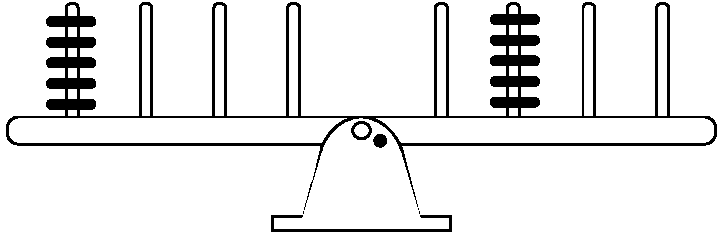
\includegraphics{graphs/baldist.pdf}
	\caption{Balance scale item; this is a so-called distance item.}
	\label{fig:balance}  
\end{center}
\end{figure}

Children in the lower grades of primary school are known to ignore the
distance dimension, and base their answer only on the number of
weights on each side.  Hence, they would typically provide the wrong
answer to these distance items.  Slightly older children do take
distance into account when responding to balance scale items, but they
only do so when the number of weights is equal on each side.  These
two strategies that children employ are known a Rule I and Rule II.
Other strategies can be teased apart by administering different items.
The \code{balance} data set that we analyse here consists of 4
distance items on a balance scale task administered to 779
participants ranging from 5 to 19 years of age.  The full set of items
consisted of 25 items; other items in the test are used to detect
other strategies that children (and young adults) employ in solving
balance scale items \citep[see][for details]{Jansen2002}. 

Similarly to the transition matrix, covariates on the prior
probabilities of the latent states (or classes in this case), are
defined by using a one-sided formula:
\begin{Schunk}
\begin{Sinput}
> data(balance)
> balance$age <- balance$age - 5
> set.seed(1)
> mod <- mix(list(d1 ~ 1, d2 ~ 1, d3 ~ 1, d4 ~ 1), data = balance, 
+     nstates = 2, family = list(multinomial(), multinomial(), 
+         multinomial(), multinomial()), respstart = c(rep(c(0.9, 
+         0.1), 4), rep(c(0.1, 0.9), 4)), prior = ~age, initdata = balance)
> fm <- fit(mod)
\end{Sinput}
\begin{Soutput}
iteration 0 logLik: -953.005 
iteration 5 logLik: -951.2919 
iteration 8 logLik: -951.2918 
\end{Soutput}
\end{Schunk}

Note here that we define a \code{mix} model instead of a \code{depmix}
models as these data form independent observations.  More formally,
\code{depmix} models extend the class of \code{mix} models by adding
the transition models.  As for fitting \code{mix} models: as can be
seen in equation~\ref{eq:Q}, the EM algorithm can be applied by simply
dropping the second summand containing the transition parameters, and 
this is implemented as such in the EM algorithms in \pkg{depmixS4}.

The summary of the \code{fit}ted model gives the following (only the
prior model is shown here):
\begin{Schunk}
\begin{Sinput}
> summary(fm, which = "prior")
\end{Sinput}
\begin{Soutput}
Mixture probabilities model 
Model of type multinomial, formula: ~age
Coefficients: 
     [,1]       [,2]
[1,]    0 -2.5182590
[2,]    0  0.5512897
Probalities at zero values of the covariates.
0.925412 0.07458803 
\end{Soutput}
\end{Schunk}

%
% add more explanation about the parameters, possibly add a plot of 
% the class membership as function of age
%

Hence at young ages, children have a high probability of incorrect 
responding in class~1, whereas the prior probability for class~2 
increases with age. 


\subsection{Fixing and constraining parameters}

Using package \pkg{Rdonlp2} by \citet{Tamura2009} or \pkg{Rsolnp}
\citet{ZZZZ???}, parameters may be fitted subject to general linear
(in-)equality constraints.  Constraining and fixing parameters is done
using the \code{conpat} argument to the \code{fit}-function, which
specifies for each parameter in the model whether it's fixed (0) or
free (1 or higher).  Equality constraints can be imposed by having two
parameters have the same number in the \code{conpat} vector.  When
only fixed values are required, the \code{fixed} argument can be used
instead of \code{conpat}, with zeroes for fixed parameters and other
values (ones e.g.) for non-fixed parameters.  Fitting the models
subject to these constraints is handled by the optimization routine
\code{donlp2}.  To be able to construct the \code{conpat} and/or
\code{fixed} vectors one needs the correct ordering of parameters
which is briefly discussed next before proceeding with an example.

\paragraph{Parameter numbering} When using the \code{conpat} and
\code{fixed} arguments, complete parameter vectors should be supplied,
i.e., these vectors should have length of the number of parameters of
the model, which can be obtained by calling \code{npar(object)}.  Note
that this is not the same as the degrees of freedom used e.g.\ in the
\code{logLik} function because \code{npar} also counts the baseline
category zeroes from the multinomial logistic models.  Parameters are
numbered in the following order:
\begin{enumerate}
	\item  the prior model parameters
	\item  the parameters for the transition models
	\item  the response model parameters per state (and subsequently
	per response in the case of multivariate time series)
\end{enumerate}

To see the ordering of parameters use the following:
\begin{Schunk}
\begin{Sinput}
> setpars(mod, value = 1:npar(mod))
\end{Sinput}
\begin{Soutput}
Initial state probabilties model 
Model of type multinomial, formula: ~age
Coefficients: 
     [,1] [,2]
[1,]    1    2
[2,]    3    4
Probalities at zero values of the covariates.
0.09893802 0.7310586 

Response model(s) for state 1 

Response model for response 1 
Model of type multinomial, formula: d1 ~ 1
Coefficients: 
     [,1] [,2]
[1,]    5    6
Probalities at zero values of the covariates.
0.001812113 0.7310586 

Response model for response 2 
Model of type multinomial, formula: d2 ~ 1
Coefficients: 
     [,1] [,2]
[1,]    7    8
Probalities at zero values of the covariates.
0.0002452428 0.7310586 

Response model for response 3 
Model of type multinomial, formula: d3 ~ 1
Coefficients: 
     [,1] [,2]
[1,]    9   10
Probalities at zero values of the covariates.
3.319001e-05 0.7310586 

Response model for response 4 
Model of type multinomial, formula: d4 ~ 1
Coefficients: 
     [,1] [,2]
[1,]   11   12
Probalities at zero values of the covariates.
4.491779e-06 0.7310586 


Response model(s) for state 2 

Response model for response 1 
Model of type multinomial, formula: d1 ~ 1
Coefficients: 
     [,1] [,2]
[1,]   13   14
Probalities at zero values of the covariates.
6.078962e-07 0.7310586 

Response model for response 2 
Model of type multinomial, formula: d2 ~ 1
Coefficients: 
     [,1] [,2]
[1,]   15   16
Probalities at zero values of the covariates.
8.22698e-08 0.7310586 

Response model for response 3 
Model of type multinomial, formula: d3 ~ 1
Coefficients: 
     [,1] [,2]
[1,]   17   18
Probalities at zero values of the covariates.
1.113401e-08 0.7310586 

Response model for response 4 
Model of type multinomial, formula: d4 ~ 1
Coefficients: 
     [,1] [,2]
[1,]   19   20
Probalities at zero values of the covariates.
1.506824e-09 0.7310586 
\end{Soutput}
\end{Schunk}

To see which parameters are fixed (by default only baseline parameters
in the multinomial logistic models for the transition models and the
initial state probabilities model):
\begin{Schunk}
\begin{Sinput}
> setpars(mod, getpars(mod, which = "fixed"))
\end{Sinput}
\begin{Soutput}
Initial state probabilties model 
Model of type multinomial, formula: ~age
Coefficients: 
     [,1]  [,2]
[1,] TRUE FALSE
[2,] TRUE FALSE
Probalities at zero values of the covariates.
0.2689414 0.2689414 

Response model(s) for state 1 

Response model for response 1 
Model of type multinomial, formula: d1 ~ 1
Coefficients: 
     [,1]  [,2]
[1,] TRUE FALSE
Probalities at zero values of the covariates.
0.2689414 0.2689414 

Response model for response 2 
Model of type multinomial, formula: d2 ~ 1
Coefficients: 
     [,1]  [,2]
[1,] TRUE FALSE
Probalities at zero values of the covariates.
0.2689414 0.2689414 

Response model for response 3 
Model of type multinomial, formula: d3 ~ 1
Coefficients: 
     [,1]  [,2]
[1,] TRUE FALSE
Probalities at zero values of the covariates.
0.2689414 0.2689414 

Response model for response 4 
Model of type multinomial, formula: d4 ~ 1
Coefficients: 
     [,1]  [,2]
[1,] TRUE FALSE
Probalities at zero values of the covariates.
0.2689414 0.2689414 


Response model(s) for state 2 

Response model for response 1 
Model of type multinomial, formula: d1 ~ 1
Coefficients: 
     [,1]  [,2]
[1,] TRUE FALSE
Probalities at zero values of the covariates.
0.2689414 0.2689414 

Response model for response 2 
Model of type multinomial, formula: d2 ~ 1
Coefficients: 
     [,1]  [,2]
[1,] TRUE FALSE
Probalities at zero values of the covariates.
0.2689414 0.2689414 

Response model for response 3 
Model of type multinomial, formula: d3 ~ 1
Coefficients: 
     [,1]  [,2]
[1,] TRUE FALSE
Probalities at zero values of the covariates.
0.2689414 0.2689414 

Response model for response 4 
Model of type multinomial, formula: d4 ~ 1
Coefficients: 
     [,1]  [,2]
[1,] TRUE FALSE
Probalities at zero values of the covariates.
0.2689414 0.2689414 
\end{Soutput}
\end{Schunk}
When fitting constraints it is useful to have good starting values 
for the parameters and hence we first fit the following model without
constraints:
\begin{Schunk}
\begin{Sinput}
> trst <- c(0.9, 0.1, 0, 0, 0.1, 0.9, 0, 0)
> mod <- depmix(list(rt ~ 1, corr ~ 1), data = speed, transition = ~Pacc, 
+     nstates = 2, family = list(gaussian(), multinomial()), trstart = trst, 
+     inst = c(0.999, 0.001))
> fm1 <- fit(mod)
\end{Sinput}
\begin{Soutput}
iteration 0 logLik: -554.2052 
iteration 5 logLik: -254.4498 
iteration 10 logLik: -249.018 
iteration 15 logLik: -248.973 
iteration 20 logLik: -248.9723 
iteration 22 logLik: -248.9723 
\end{Soutput}
\end{Schunk}

After this, we use the fitted values from this model to constrain the
regression coefficients on the transition matrix (parameters numbers~6
and~10):
\begin{Schunk}
\begin{Sinput}
> conpat <- c(0, 1, rep(c(0, 1), 4), 1, 1, 0, 1, 1, 1, 0, 1)
> conpat[6] <- conpat[10] <- 2
> fm2 <- fit(fm1, equal = conpat)
\end{Sinput}
\begin{Soutput}
Rdonlp2 - a wrapper library for "DONLP2 (C) Peter Spellucci"


Loading required package: Rsolnp (version 0.3)
    1 fx=   0.000000e+00 upsi=  6.7e+00 b2n= -1.0e+00 umi=  0.0e+00 nr   1 si-1
    2 fx=   2.640133e+02 upsi=  0.0e+00 b2n=  2.1e+01 umi=  0.0e+00 nr   1 si-1
    3 fx=   2.636388e+02 upsi=  0.0e+00 b2n=  5.4e+01 umi=  0.0e+00 nr   1 si-1
    4 fx=   2.587645e+02 upsi=  0.0e+00 b2n=  2.7e+02 umi=  0.0e+00 nr   1 si-1
    5 fx=   2.528471e+02 upsi=  0.0e+00 b2n=  1.2e+02 umi=  0.0e+00 nr   1 si-1
    6 fx=   2.523984e+02 upsi=  0.0e+00 b2n=  9.6e+01 umi=  0.0e+00 nr   1 si-1
    7 fx=   2.523907e+02 upsi=  0.0e+00 b2n=  9.5e+01 umi=  0.0e+00 nr   1 si-1
    8 fx=   2.522057e+02 upsi=  0.0e+00 b2n=  9.2e+01 umi=  0.0e+00 nr   1 si-1
    9 fx=   2.515501e+02 upsi=  0.0e+00 b2n=  5.8e+01 umi=  0.0e+00 nr   1 si-1
   10 fx=   2.510856e+02 upsi=  0.0e+00 b2n=  5.2e+01 umi=  0.0e+00 nr   1 si-1
   11 fx=   2.507418e+02 upsi=  0.0e+00 b2n=  7.2e+01 umi=  0.0e+00 nr   1 si-1
   12 fx=   2.503033e+02 upsi=  0.0e+00 b2n=  1.9e+01 umi=  0.0e+00 nr   1 si-1
   13 fx=   2.502725e+02 upsi=  0.0e+00 b2n=  9.8e-01 umi=  0.0e+00 nr   1 si-1
   14 fx=   2.502723e+02 upsi=  0.0e+00 b2n=  1.5e-01 umi=  0.0e+00 nr   1 si-1
   15 fx=   2.502723e+02 upsi=  0.0e+00 b2n=  3.1e-02 umi=  0.0e+00 nr   1 si-1
   16 fx=   2.502723e+02 upsi=  0.0e+00 b2n=  4.1e-02 umi=  0.0e+00 nr   1 si-1
   17 fx=   2.502723e+02 upsi=  0.0e+00 b2n=  6.3e-02 umi=  0.0e+00 nr   1 si-1
   18 fx=   2.502723e+02 upsi=  0.0e+00 b2n=  2.9e-02 umi=  0.0e+00 nr   1 si-1
   19 fx=   2.502723e+02 upsi=  0.0e+00 b2n=  4.1e-03 umi=  0.0e+00 nr   1 si-1
   20 fx=   2.502723e+02 upsi=  0.0e+00 b2n=  1.4e-04 umi=  0.0e+00 nr   1 si-1
   21 fx=   2.502723e+02 upsi=  0.0e+00 b2n=  4.3e-03 umi=  0.0e+00 nr   1 si-1
   22 fx=   2.502723e+02 upsi=  0.0e+00 b2n=  9.4e-02 umi=  0.0e+00 nr   1 si-1
   23 fx=   2.502723e+02 upsi=  0.0e+00 b2n=  1.1e-01 umi=  0.0e+00 nr   1 si-1
   24 fx=   2.502723e+02 upsi=  0.0e+00 b2n=  1.1e-01 umi=  0.0e+00 nr   1 si-1
   25 fx=   2.502723e+02 upsi=  0.0e+00 b2n=  2.7e-02 umi=  0.0e+00 nr   1 si-1
   26 fx=   2.502723e+02 upsi=  0.0e+00 b2n=  4.6e-02 umi=  0.0e+00 nr   1 si-1
   27 fx=   2.502723e+02 upsi=  0.0e+00 b2n=  2.0e-03 umi=  0.0e+00 nr   1 si-1
   28 fx=   2.502723e+02 upsi=  0.0e+00 b2n=  2.0e-02 umi=  0.0e+00 nr   1 si-1
   29 fx=   2.502723e+02 upsi=  0.0e+00 b2n=  4.9e-02 umi=  0.0e+00 nr   1 si-1
   30 fx=   2.502723e+02 upsi=  0.0e+00 b2n=  1.2e-01 umi=  0.0e+00 nr   1 si-1
   31 fx=   2.502723e+02 upsi=  0.0e+00 b2n=  1.2e-01 umi=  0.0e+00 nr   1 si-1
   32 fx=   2.502723e+02 upsi=  0.0e+00 b2n=  1.2e-01 umi=  0.0e+00 nr   1 si-1
   33 fx=   2.502723e+02 upsi=  0.0e+00 b2n=  1.2e-01 umi=  0.0e+00 nr   1 si-1
   34 fx=   2.502723e+02 upsi=  0.0e+00 b2n=  1.2e-01 umi=  0.0e+00 nr   1 si-1
   35 fx=   2.502723e+02 upsi=  0.0e+00 b2n=  1.2e-01 umi=  0.0e+00 nr   1 si-1
   36 fx=   2.502723e+02 upsi=  0.0e+00 b2n=  1.1e-01 umi=  0.0e+00 nr   1 si-1
   37 fx=   2.502723e+02 upsi=  0.0e+00 b2n=  1.1e-01 umi=  0.0e+00 nr   1 si-1
   38 fx=   2.502723e+02 upsi=  0.0e+00 b2n=  1.5e-02 umi=  0.0e+00 nr   1 si-1


     n=        11    nlin=         1    nonlin=         0

  epsx= 1.000e-05 sigsm= 1.490e-08

startvalue
  1.1073464e+01  -4.2226665e+00   9.1333225e+00  -3.3734642e+00   1.5804664e+01 
  5.5217147e+00   2.0291526e-01   1.0305078e-01   6.3937023e+00   2.3735863e-01 
  2.2456760e+00 

  eps=  2.22e-16  tol= 2.23e-308 del0=  1.00e+00 delm=  1.00e-06 tau0=  1.00e+00
  tau=  1.00e-01   sd=  1.00e-01   sw=  3.67e-11  rho=  1.00e-06 rho1=  1.00e-10
 scfm=  1.00e+04  c1d=  1.00e-02 epdi=  1.00e-08
  nre=        11 anal=         0
taubnd=  1.00e+00 epsfcn=  1.00e-16 difftype=2

 termination reason:
 KT-conditions satisfied, no further correction computed
 evaluations of f                          149
 evaluations of grad f                      38
 evaluations of constraints                150
 evaluations of grads of constraints         0
 final scaling of objective           2.578752e+00
 norm of grad(f)                      5.469760e-01
 lagrangian violation                 3.850303e-06
 feasibility violation                0.000000e+00
 dual feasibility violation           0.000000e+00
 optimizer runtime sec's              1.020294e+02


 optimal value of f =   2.50272256745793e+02

 optimal solution  x =
  1.66634775085811e+01 -5.33950908658836e+00  1.26660713921942e+01
 -2.42709046868253e+00  1.26660713921942e+01  5.52688670523495e+00
  2.09034923220784e-01  1.03019938087600e-01  6.39615051769729e+00
  2.36133701083779e-01  2.27764355098866e+00

  multipliers are relativ to scf=1
  nr.    constraint     multiplier norm(grad) or 1 
    1   1.0000000e+20    0.0000000e+00 
    2   1.0000000e+20    0.0000000e+00 
    3   1.0000000e+20    0.0000000e+00 
    4   1.0000000e+20    0.0000000e+00 
    5   1.0000000e+20    0.0000000e+00 
    6   1.0000000e+20    0.0000000e+00 
    7   1.0000000e+20    0.0000000e+00 
    8   1.0000000e+20    0.0000000e+00 
    9   1.0000000e+20    0.0000000e+00 
   10   1.0000000e+20    0.0000000e+00 
   11   1.0000000e+20    0.0000000e+00 
   12   1.0000000e+20    0.0000000e+00 
   13   1.0000000e+20    0.0000000e+00 
   14   1.0000000e+20    0.0000000e+00 
   15   1.0000000e+20    0.0000000e+00 
   16   1.0000000e+20    0.0000000e+00 
   17   1.0000000e+20    0.0000000e+00 
   18   1.0000000e+20    0.0000000e+00 
   19   1.0000000e+20    0.0000000e+00 
   20   1.0000000e+20    0.0000000e+00 
   21   1.0000000e+20    0.0000000e+00 
   22   1.0000000e+20    0.0000000e+00 
   23   0.0000000e+00    3.8677046e-01    1.4142136e+00
   24   0.0000000e+00    0.0000000e+00 

 evaluations of restrictions and their gradients
 (   150,     0)
 last estimate of cond.nr. of active gradients   1.000e+00

 last estimate of cond.nr. of approx.  hessian   3.187e+06
iterative steps total              38
# of restarts                       1
# of full regular updates          36
# of updates                       36
# of regularized full SQP-steps     0
\end{Soutput}
\end{Schunk}

Using \code{summary} on the fitted model shows that the regression 
coefficients are now estimated at the same value of 12.66. The function
\code{llratio} computes the likelihood ratio $\chi^2$-statistic and the
associated $p$-value with appropriate degrees of freedom for testing the
tenability of constraints \citep{Dannemann2007}. Note that these arguments 
provide the possibility for arbitrary 
constraints, also between, e.g., a multinomial regression coefficient 
for the transition matrix and the mean of a Gaussian response model. 
Whether such constraints make sense is hence the responsibility of 
the user. 

\section[Extending depmixS4]{Extending \pkg{depmixS4}}

The \pkg{depmixS4} package was designed with the aim of making it
relatively easy to add new response distributions (as well as possibly
new prior and transition models).  To make this possible, the EM
routine simply calls the \code{fit} methods of the separate response
models without needing access to the internal workings of these
routines.  Referring to equation~\ref{eq:Q}, the EM algorithm calls
separate fit functions for each part of the model, the prior
probability model, the transition models, and the response models.  As
a consequence, adding user-specified response models is
straightforward.

User-defined distributions should extend the \code{response}-class and
have the following slots:
\begin{enumerate}
	\item y: the response variable
	\item x: the design matrix, possibly only an intercept
	\item paramaters: a named list with the coefficients and possibly 
	other parameters, e.g., the standard deviation in the Gaussian 
	response model
	\item fixed: a vector of logicals indicating whether parameters are 
	fixed
	\item npar: numerical indicating the number of parameters of the model
\end{enumerate}

In the \code{speed} data example, it may be more appropriate to model
the response times with an exgaus rather than a Gaussian distribution.
To do so, we first define an exgaus-class extending the
response-class:
\begin{Schunk}
\begin{Sinput}
> setClass("exgaus", contains = "response")
\end{Sinput}
\begin{Soutput}
[1] "exgaus"
\end{Soutput}
\end{Schunk}

The so-defined class now needs a number of methods: 
\begin{enumerate}
	\item constructor: function to create instances of the class 
	with starting values
	\item show method: to print the model to the terminal
	\item dens: the function that computes the density of the responses
	\item getpars and setpars: to get and set parameters 
	\item predict: to generate predict'ed values 
	\item fit: function to fit the model using posterior weights (used 
	by the EM algorithm)
\end{enumerate}

Only the constructor and the fit methods are provided here; the
complete code can be found in the help file of the \code{makeDepmix}
function.  The \code{exgaus} example uses the \pkg{gamlss} and
\pkg{gamlss.distr} packages
\citep{Stasinopoulos2009a,Stasinopoulos2009b} for computing the
\code{dens}ity and for \code{fit}ting the parameters.

The constructor method return an object of class \code{exgaus}, and is
defined as follows:
\begin{Schunk}
\begin{Sinput}
> setGeneric("exgaus", function(y, pstart = NULL, fixed = NULL, 
+     ...) standardGeneric("exgaus"))
\end{Sinput}
\begin{Soutput}
[1] "exgaus"
\end{Soutput}
\begin{Sinput}
> require(gamlss)
\end{Sinput}
\begin{Soutput}
 **********   GAMLSS Version 3.0-1 ********** 
For more on GAMLSS look at http://www.gamlss.com/ 
Type gamlssNews() to see new features/changes/bug fixes.
\end{Soutput}
\begin{Sinput}
> require(gamlss.dist)
> setMethod("exgaus", signature(y = "ANY"), function(y, pstart = NULL, 
+     fixed = NULL, ...) {
+     y <- matrix(y, length(y))
+     x <- matrix(1)
+     parameters <- list()
+     npar <- 3
+     if (is.null(fixed)) 
+         fixed <- as.logical(rep(0, npar))
+     if (!is.null(pstart)) {
+         if (length(pstart) != npar) 
+             stop("length of 'pstart' must be ", npar)
+         parameters$mu <- pstart[1]
+         parameters$sigma <- log(pstart[2])
+         parameters$nu <- log(pstart[3])
+     }
+     mod <- new("exgaus", parameters = parameters, fixed = fixed, 
+         x = x, y = y, npar = npar)
+     mod
+ })
\end{Sinput}
\begin{Soutput}
[1] "exgaus"
\end{Soutput}
\end{Schunk}



\begin{Schunk}
\begin{Soutput}
[1] "dens"
\end{Soutput}
\begin{Soutput}
[1] "getpars"
\end{Soutput}
\begin{Soutput}
[1] "setpars"
\end{Soutput}
\begin{Soutput}
[1] "predict"
\end{Soutput}
\end{Schunk}


The \code{fit} method is defined as follows: 
\begin{Schunk}
\begin{Sinput}
> setMethod("fit", "exgaus", function(object, w) {
+     if (missing(w)) 
+         w <- NULL
+     y <- object@y
+     fit <- gamlss(y ~ 1, weights = w, family = exGAUS(), control = gamlss.control(n.cyc = 100, 
+         trace = FALSE), mu.start = object@parameters$mu, sigma.start = exp(object@parameters$sigma), 
+         nu.start = exp(object@parameters$nu))
+     pars <- c(fit$mu.coefficients, fit$sigma.coefficients, fit$nu.coefficients)
+     object <- setpars(object, pars)
+     object
+ })
\end{Sinput}
\begin{Soutput}
[1] "fit"
\end{Soutput}
\end{Schunk}

The \code{fit} method defines a \code{gamlss} model with 
only an intercept to be estimated and then sets the fitted parameters 
back into their respective slots in the `exgaus' object. See the help 
for \code{gamlss.distr} for interpretation of these parameters. 

After defining all the necessary methods for the new response model, 
we can  now define the dependent mixture model using this reponse model. 
The function \code{makeDepmix} is included in \pkg{depmixS4} to have 
full control over model specification, and we need it here. 

We first create all the response models that we need as a double list: 
\begin{Schunk}
\begin{Sinput}
> rModels <- list(list(exgaus(speed$rt, pstart = c(5, 0.1, 0.1)), 
+     GLMresponse(formula = corr ~ 1, data = speed, family = multinomial(), 
+         pstart = c(0.5, 0.5))), list(exgaus(speed$rt, pstart = c(6, 
+     0.1, 0.1)), GLMresponse(formula = corr ~ 1, data = speed, 
+     family = multinomial(), pstart = c(0.1, 0.9))))
\end{Sinput}
\end{Schunk}

Next, we define the transition and prior probability models using the 
\code{transInit} function (which produces a transInit model, which also extends 
the response class): 
\begin{Schunk}
\begin{Sinput}
> trstart = c(0.9, 0.1, 0.1, 0.9)
> transition <- list()
> transition[[1]] <- transInit(~Pacc, nst = 2, data = speed, pstart = c(0.9, 
+     0.1, 0, 0))
> transition[[2]] <- transInit(~Pacc, nst = 2, data = speed, pstart = c(0.1, 
+     0.9, 0, 0))
> inMod <- transInit(~1, ns = 2, pstart = c(0.1, 0.9), data = data.frame(1))
\end{Sinput}
\end{Schunk}

Finally, we put everything together using \code{makeDepmix} and fit 
the model: 
\begin{Schunk}
\begin{Sinput}
> mod <- makeDepmix(response = rModels, transition = transition, 
+     prior = inMod, stat = FALSE)
> fm <- fit(mod)
\end{Sinput}
\begin{Soutput}
iteration 0 logLik: -265.0144 
iteration 5 logLik: -243.4716 
iteration 10 logLik: -232.3604 
iteration 15 logLik: -232.2586 
iteration 20 logLik: -232.2537 
iteration 25 logLik: -232.2528 
iteration 30 logLik: -232.2527 
iteration 35 logLik: -232.2526 
iteration 40 logLik: -232.2526 
iteration 43 logLik: -232.2526 
\end{Soutput}
\end{Schunk}

Using \code{summary} will print the fitted parameters.  Note that the
use of \code{makeDepmix} allows the possibility of, say, fitting a
Gaussian in one state and an exgaus distribution in another state.
Note also that according to the AIC and BIC, the model with the exgaus
describes the data much better than the same model in which the
response times are modeled as gaussian.


\section[Conclusions and future work]{Conclusions \& future work}

\pkg{depmixS4} provides a flexible framework for fitting dependent
mixture models for a large variety of response distributions.  It can
also fit latent class regression and finite mixture models, although
it should be noted that more specialized packages are available for
this such as \pkg{FlexMix} \citep{Leisch2004}.  The package is
intended for modeling of (individual) time series data with the aim of
characterizing the transition processes underlying the data.  The
possibility to use covariates on the transition matrix greatly
enhances the flexibility of the model.  The EM algorithm uses a very
general interface that allows easy addition of new response models.

We are currently working on implementing the gradients for response
and transition models with two goals in mind.  First, to speed up
(constrained) parameter optimization using \pkg{Rdonlp2}.  Second,
analytic gradients are useful in computing the Hessian of the
estimated parameters so as to arrive at standard errors for those.  We
are also planning to implement goodness-of-fit statistics
\citep{Titman2008}, and automatic generation of starting values.


\section*{Acknowledgements} 

Ingmar Visser was supported by an EC Framework 6 grant, project 516542
(NEST).  Maarten Speekenbrink was supported by the ESRC Centre for
Economic Learning and Social Evolution (ELSE).  Han van der Maas
provided the speed-accuracy data \cite{Dutilh2009} and thereby
neccessitated implementing models with time-dependent covariates.
Brenda Jansen provided the balance scale data set \citep{Jansen2002}
which was the perfect opportunity to test the covariates on the prior
model parameters.  The examples in the help files use both of these
data sets.


\bibliography{all,ingmar}

\end{document}


